\section*{Overview of process}
Different prototypes were used to decide, how the program should interact with the user and how the final user interface should be designed. In the following sections three different prototypes will be shown along with their work process and an explanation of related decision making.
The first prototypes were drawings on a blackboard or a piece of paper that were later converted to an HTML prototype (see section  \vref{program_tools_html_css}). In this process three group members designed the first prototype and presented it to the group. The group discussed points of improvements which led to a new design of the prototype. The HTML prototype was shown to kindergarten teacher Kristine Niss-Henriksen, in the second interview which is summarized in appendix \vref{sec_interview_birken}.

\section{The first prototypes}
After the first prototype was presented, each page was drawn on to a blackboard where the changes were more manageable. One of the first blackboard designs was the page ``Settings'', which contained information such as the child's name and abilities, shown in Figure \vref{fig:firstProto}. This is a primitive design with two menus, one horizontal and one vertical, the horizontal axis has all children and groups of children, the vertical axis has all the applications on a child's device, that the user can administer. This menu will be further explained in the section\vref{menus}. 

\begin{figure}[!ht]
	\centering
		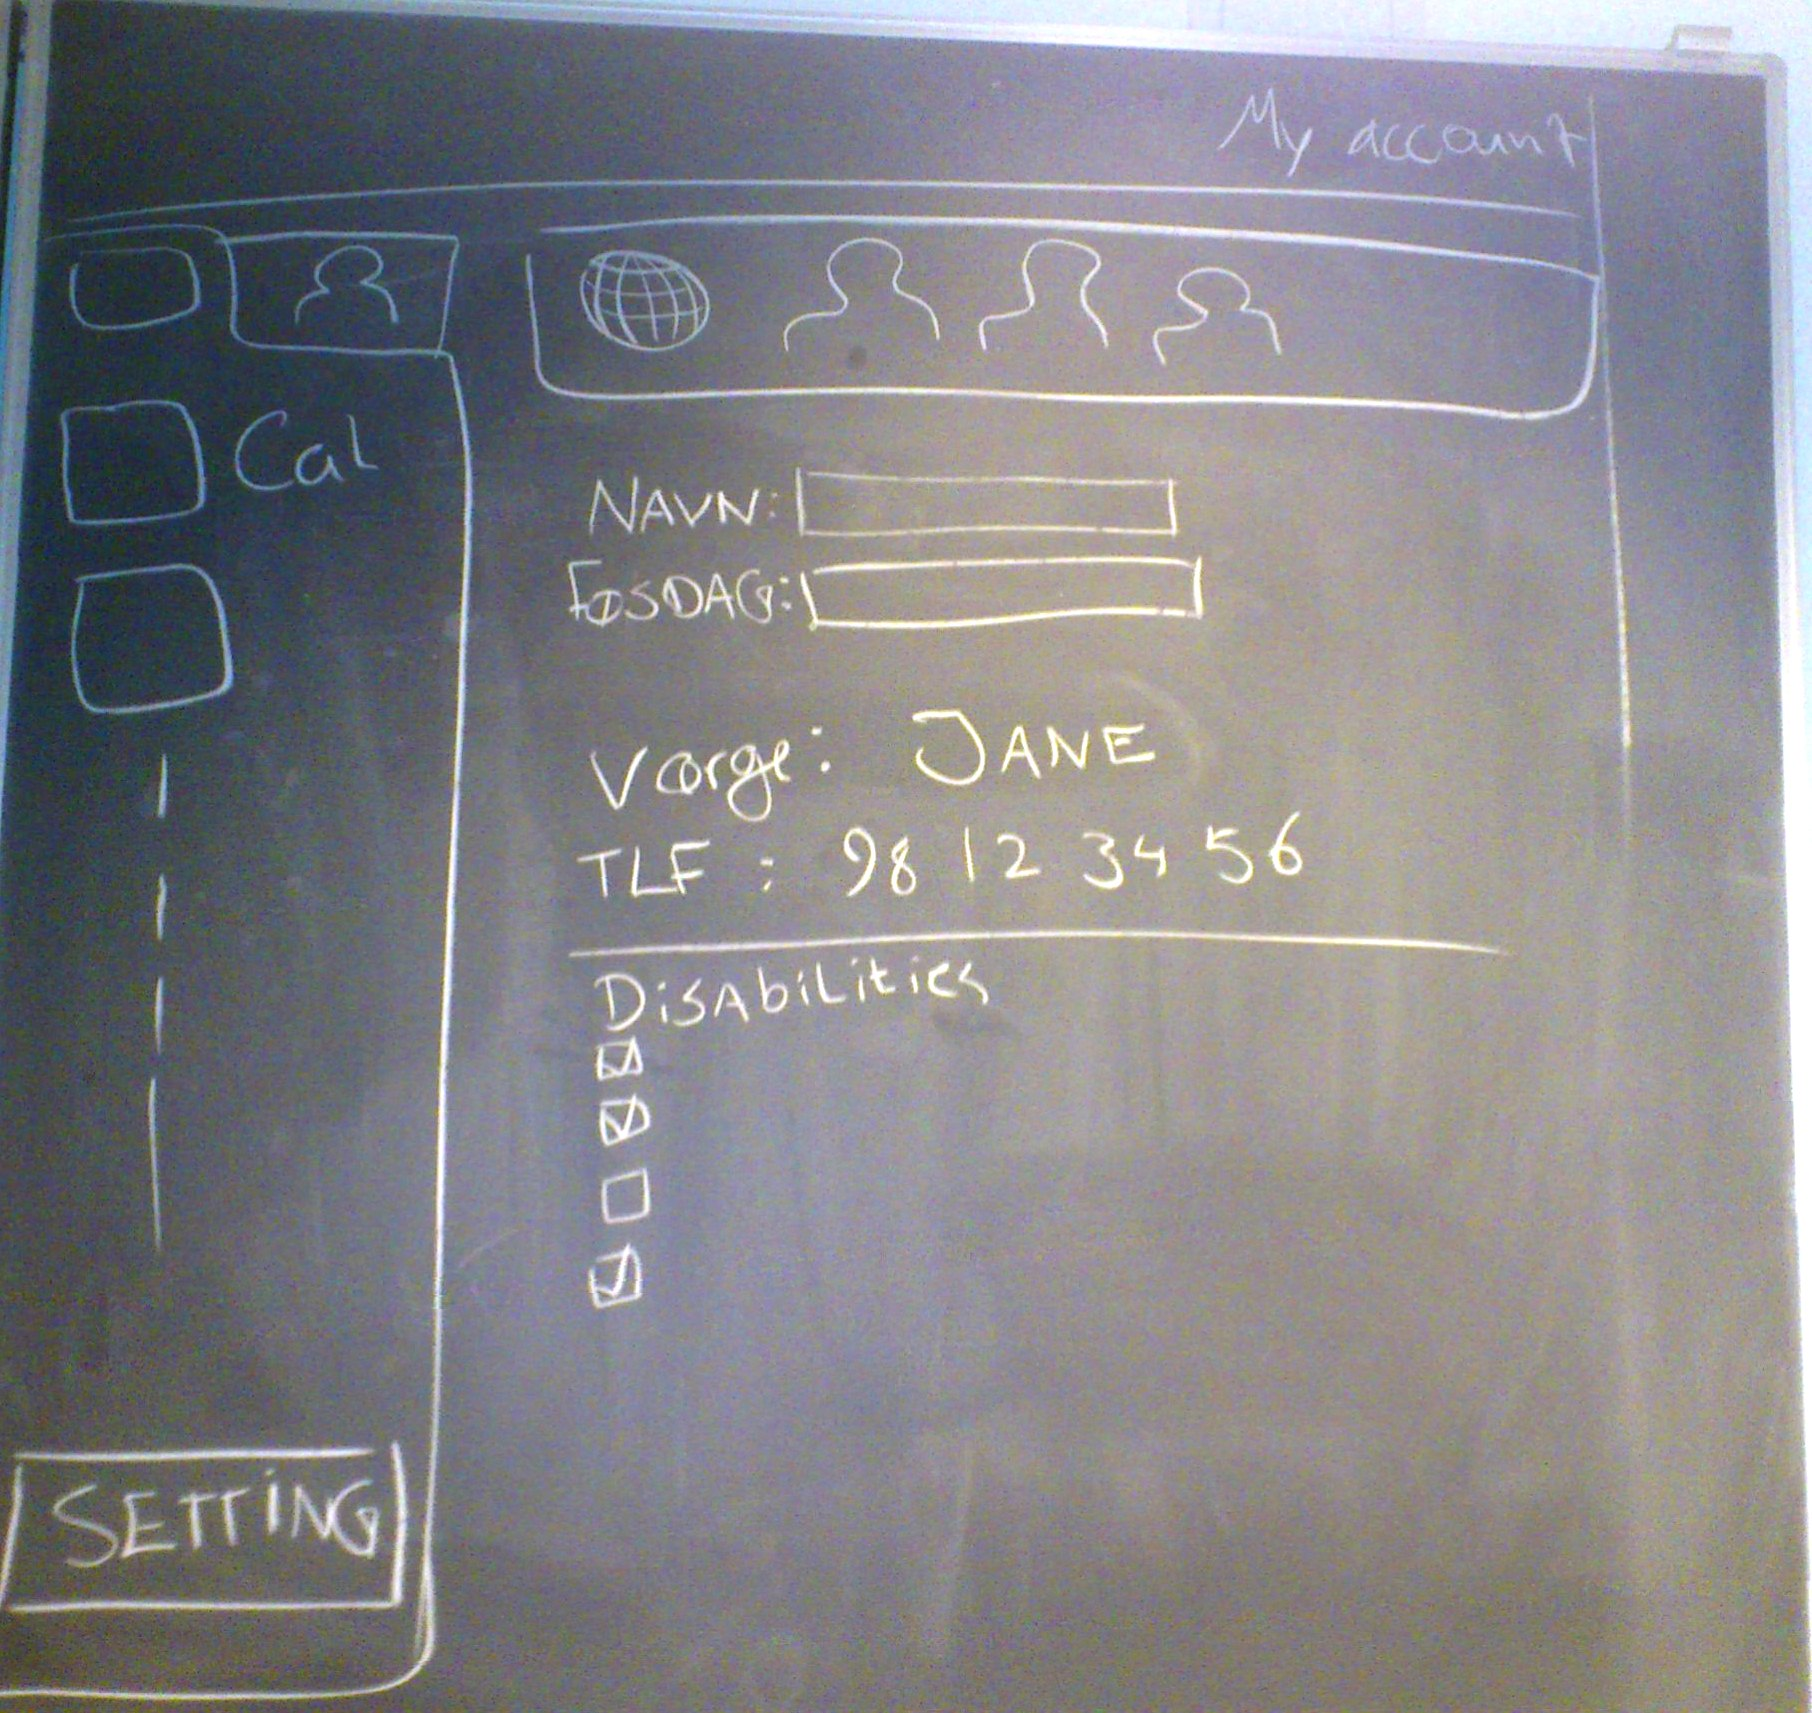
\includegraphics[width=0.60\textwidth]{img/firstproto.jpg}
	\caption{Black board design of the interface}
	\label{fig:firstProto}
\end{figure}


The group members disagreed on how to get into the ``Settings'' page in the first design. Reason being that the user would have to choose a child in the top horizontal menu and the press the ``Settings'' button in the vertical menu, which is located among GIRAF applications. Especially the location and the naming of the ``Settings'' button were discussed because the user could get the impression that they administer a child like an application and thereby creating confusion. To solve this it was suggested that this page should be in ``My Account'' instead; where the user would also be able to change their own personal information. The prototype design was not changed, and ``Settings'' page was never implemented.

\section{The HTML prototype}
For the second interview with Kristine Niss-Henriksen, an HTML prototype was made from the primitive prototypes. The Figure \vref{fig:contactbook} is two screen shoots from the child Jack's contact book where the right side of the figure is a light box with an entry from the contact book. The contact book is inspired by a calendar because, for each date, it can have entries which the user can click on. When clicked, a light box pops up that contains the message and pictures. If the user has not seen the message before, the signal ``Ny!'' in the right side should be visible. The user is able to fold and unfold the entries for each date, to see or hide the entries in the contact book. 

\begin{figure}[!ht]
	\centering
		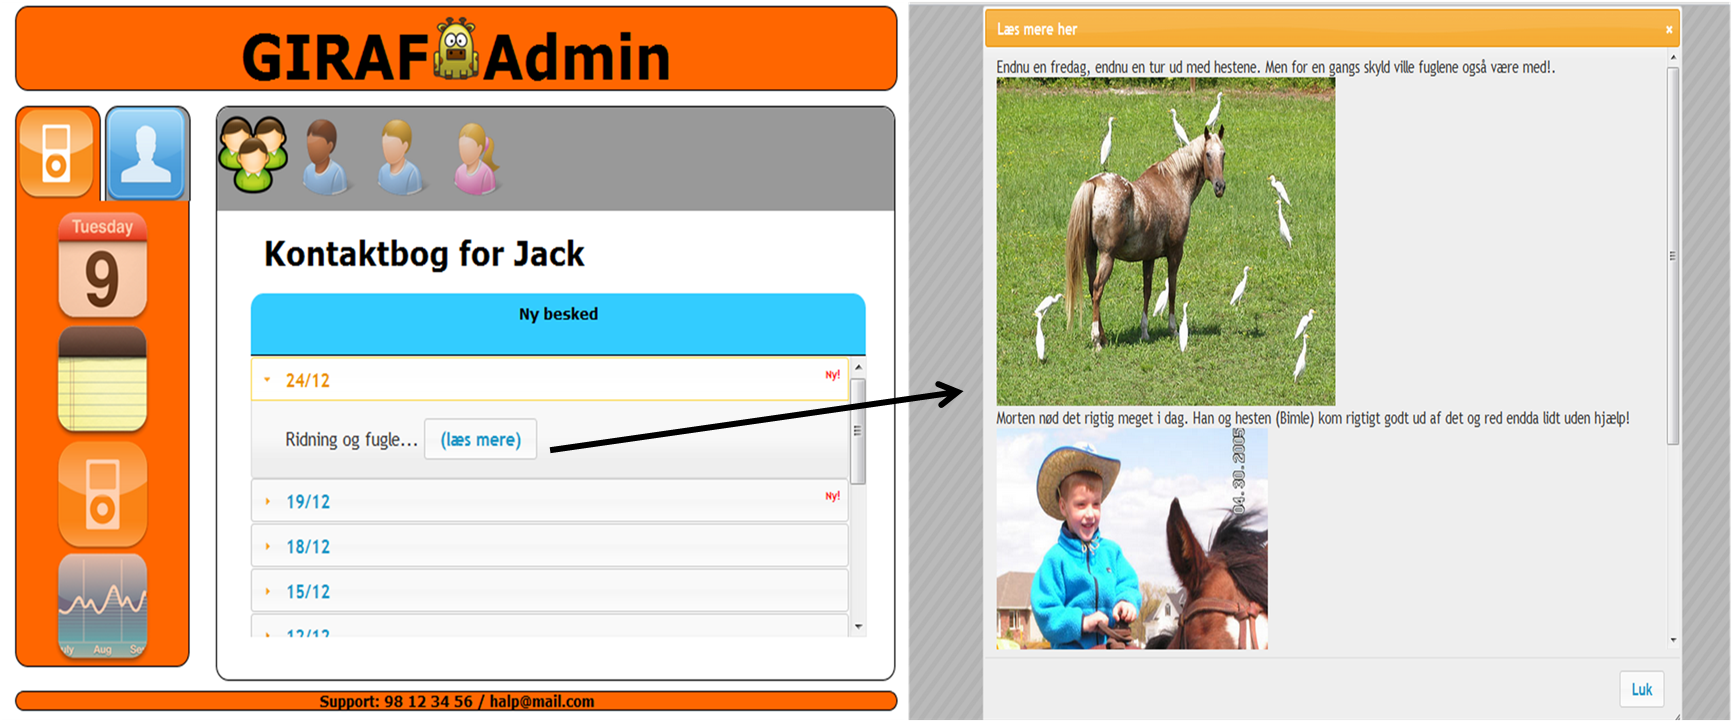
\includegraphics[angle=90,width=0.65\textwidth]{img/contactbook.png}
	\caption{Prototype of the contact book and the light box with an entry}
	\label{fig:contactbook}
\end{figure}

\subsection{The menus}
\label{menus}
As it was pointed out earlier the GIRAF applications' administrators are represented on the vertical menu, as an icon that should identify the application administrator. The children's devices are represented on the horizontal menu where the single child's device is identified from a picture and the group is identified by an icon representing a group of children. However this representation can be mirrored such that the children's devices are represented on the vertical menu and the applications are represented on the horizontal menu, which is shown in Figure \vref{fig:menus}. The black circle indicates which of the menus is represented in the vertical menu. This menu was not implemented because it would take too much of the space on the screen, and it could also be a confusing navigation path for the user, without gaining any new functionality. In the next prototype this menu was replaced with two vertical menus side by side.

\begin{figure}[!ht]
	\centering
		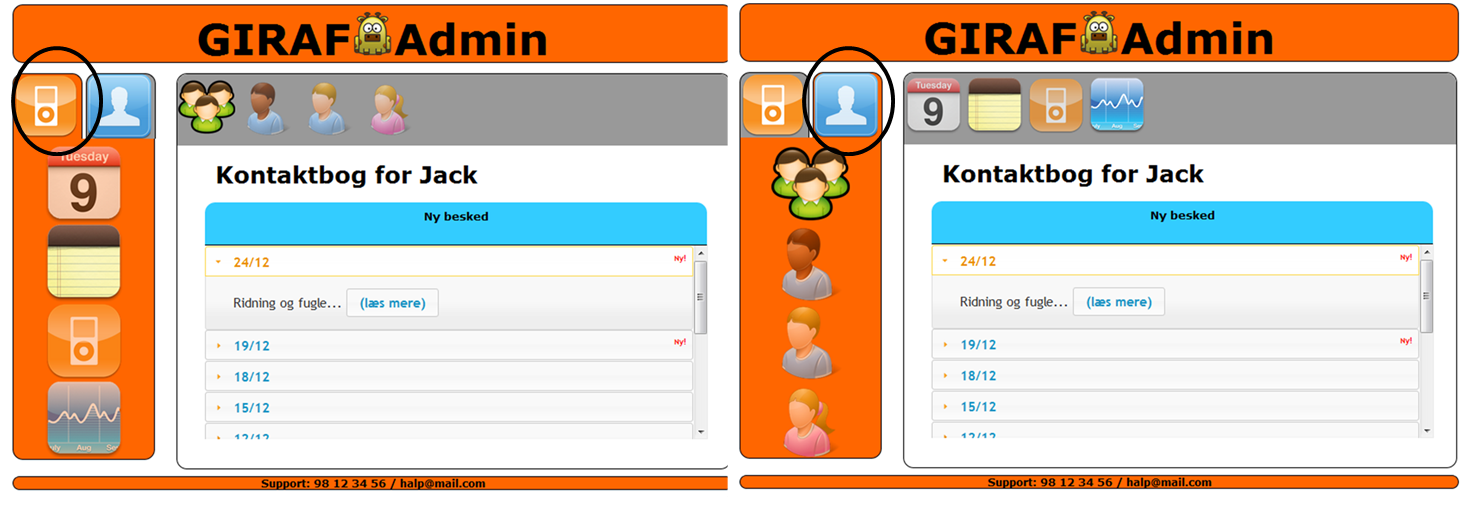
\includegraphics[width=1.00\textwidth]{img/menus.png}
	\caption{The menus in the HTML prototype}
	\label{fig:menus}
\end{figure}


\subsection{Evaluation of the HTML prototype}
In the second interview, see appendix \vref{sec_interview_birken}, with Kristine Niss-Henriksen from Birken we introduced the HTML prototype to her. In general she liked the design but suggested that the icon for a child should be a photo of the child itself, which also was indented. She also expressed a need for a way to reply to a message, which would be useful since it is used both by the parents and kindergarten teachers. Kristine said: ``[communication] \emph{It goes in both directions. The parents write in the contact book in the morning and we write during the afternoon which then can result in a longer dialog between the parties.}'' in appendix \vref{sec_interview_birken} [12:24]. The reply function was then included during the implementation. 

She tried to create a new message and wondered if there was some sort of spell checking in the text field, after realising that this was not the case, she suggested it to be added. We consider this to be a minor improvement, that could be implemented later. 

She saw two versions of the contact book, the first being able to contain several pictures and text; while the other contained text but only one picture - see Figure \vref{fig:createmessage}. She said: "\emph{both can work - because what we do when we are on a trip and add pictures is that we always write something to the picture, but also some general information about the day's events. ... What I think, is that you should somehow be able to separate the text}"\ref{sec_interview_birken} [24:50]. This functionality was added in the contact book during implementation, a text label can be attached to each picture and there is also a text field for general information about the day. 

\begin{figure}[!ht]
	\centering
		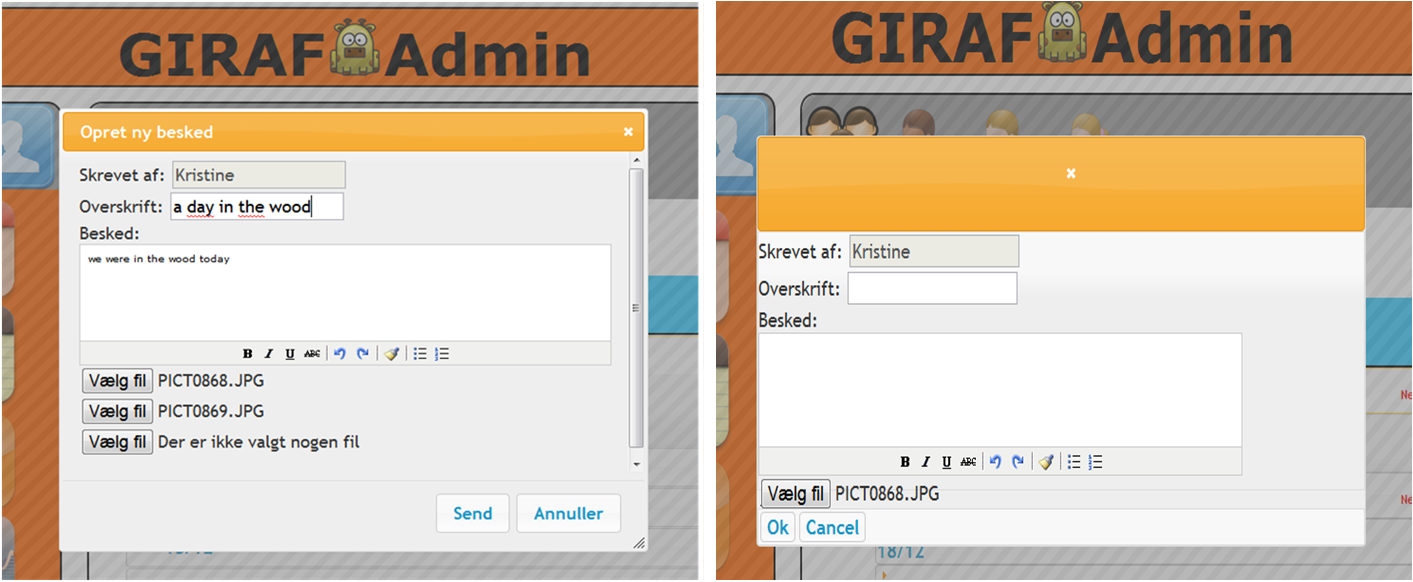
\includegraphics[angle=90,width=0.65\textwidth]{img/createmessage.png}
	\caption{Create message from the contact book in two versions}
	\label{fig:createmessage}
\end{figure}

In the beginning of the interview, she showed us a standard information sheet that contained the child's name, the parents' name and contact information. The current contact book has this sheet on the first page and Kristine thought that it also should be included in the digital contact book. However, the sheet will not be placed within the contact book.
She also suggested that the information sheet could be implemented as a button among the other applications' administrators, much like the ``Settings'' button, from the first prototype. We chose to place the information sheet among other information about the child in a specific location. 

During the interview she expressed that they rarely edit pictures before printing, but if they were to upload a picture in a message and easily had access to; rotation, crop and resize, she would likely use it. If these ideas were to be implemented, she would also need an undo function. These functions were considered ``nice to have'' and therefore were not prioritised highly in implementation.
From our prototype it was not clear that it would be a closed system, where the kindergarten teachers and parents would have to login before they would be able see or write in the contact book. She considered this to be very important because the information in the contact book might be very sensitive. The Personal Data Protection Act covers this area. 

Kristine pointed out that a child always gets copy of his/hers contact book, when moving out of the kindergarten. If the digital contact book were to be used instead, this tradition would be lost. Therefore she suggested that the user e.g. should be able to print the logs from the contact book so they would not be lost afterwards, since Birken are not allowed to have information indefinitely because of the Personal Data Protection Act. The solution to this problem should be studied further.

After the interview, we wanted to have a start page with general information about meetings and news from Birken to the parents. Kristine first talked about this information in relation to the calendar which is only represented by an icon in the prototype, but that calendar was designed for the child, so the other solution was preferred.

\section{The last paper prototype}
In the last paper prototype, the menu has changed to two vertical menus, where the user needs to click on an application, a child and then press a go-button to get the application settings for that child. This is shown in the Figure \vref{fig:calendar} in which the application aSchedule's administrator for Jack is called, however we never implemented an administrator module for aSchedule. When this design was evaluated, it was considered easier to understand and implement if the user should choose a child or a group of children first and then choose an application. Reason being that the applications' administrator depends on the installed applications on the child's device. The GO-button was considered unnecessary and therefore abandoned, along with the button ``Settings'', as mentioned earlier.

\begin{figure}[!ht]
	\centering
		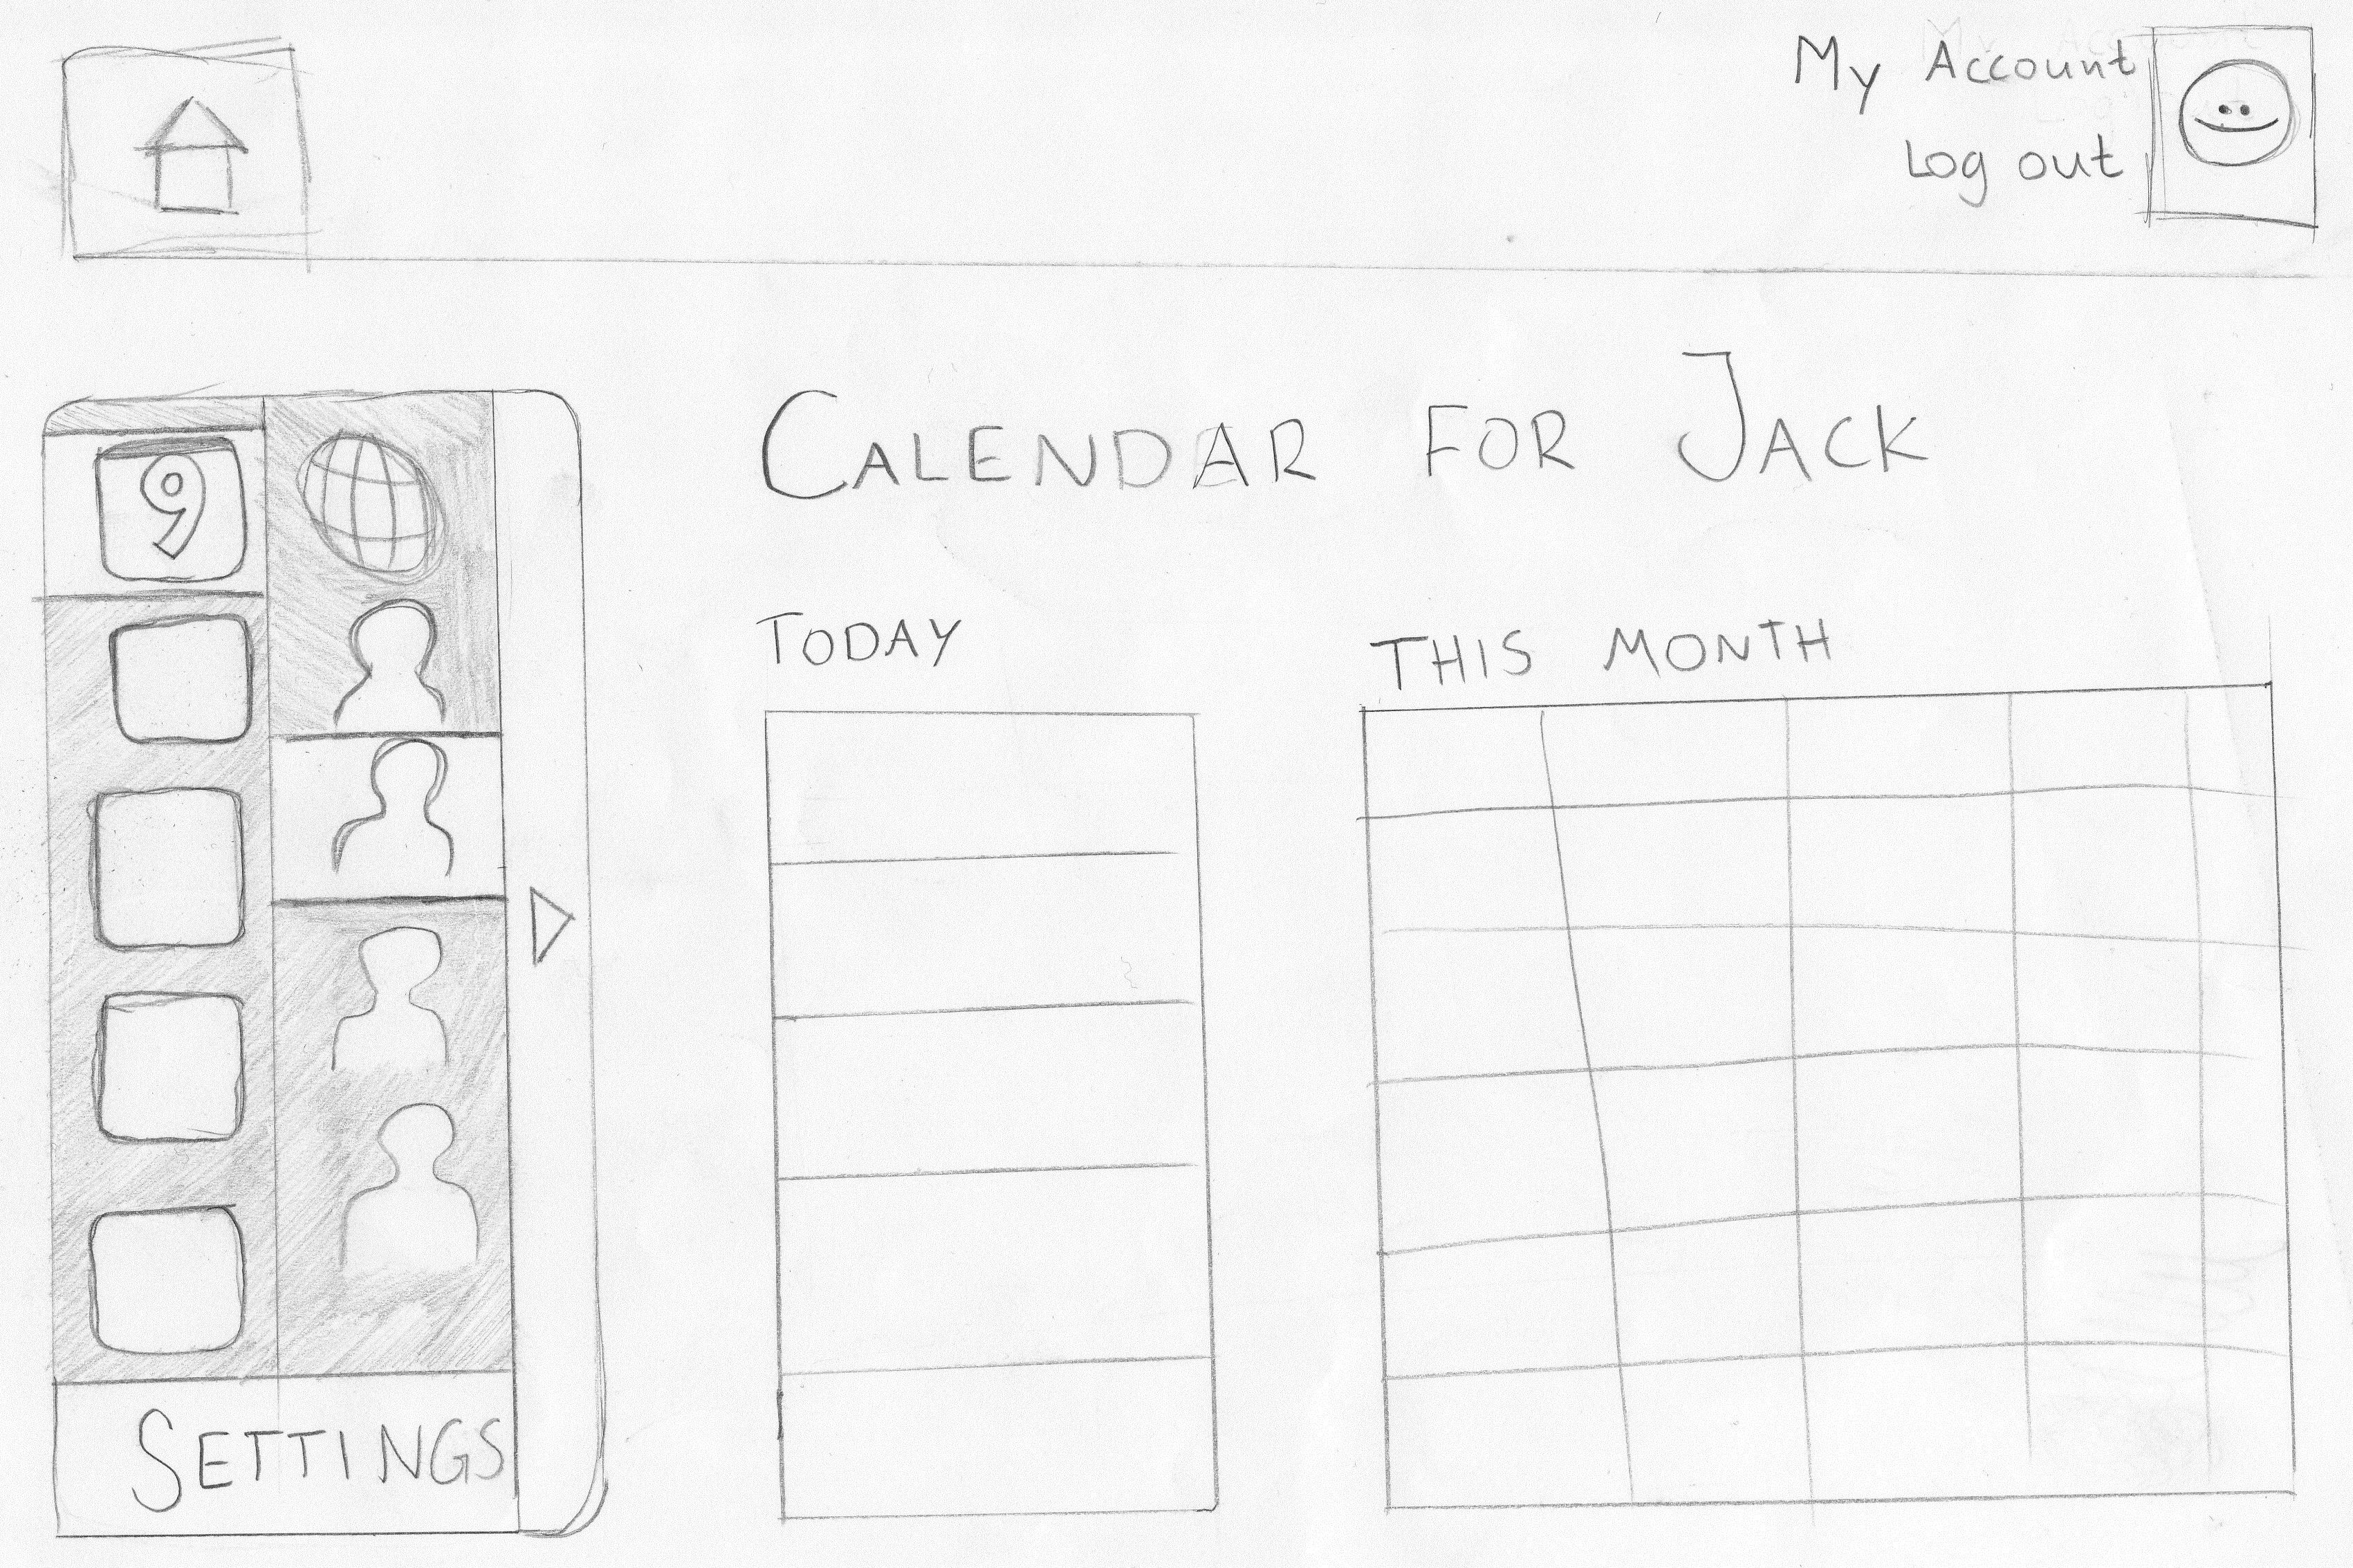
\includegraphics[width=1.00\textwidth]{img/calendar.jpg}
	\caption{Paper prototype of aSchedule's administration application and general design}
	\label{fig:calendar}
\end{figure}

  
In the top-left corner of the prototype is the homepage button which should contain general information and news from the kindergarten, this was one of the changes made as a result of the interview with Kristine. In the top-right corner should be a logout button and a ``My Account'' button, which leads to personal information, shown in Figure \vref{fig:myAccount}. 
\begin{figure}[!ht]
	\centering
		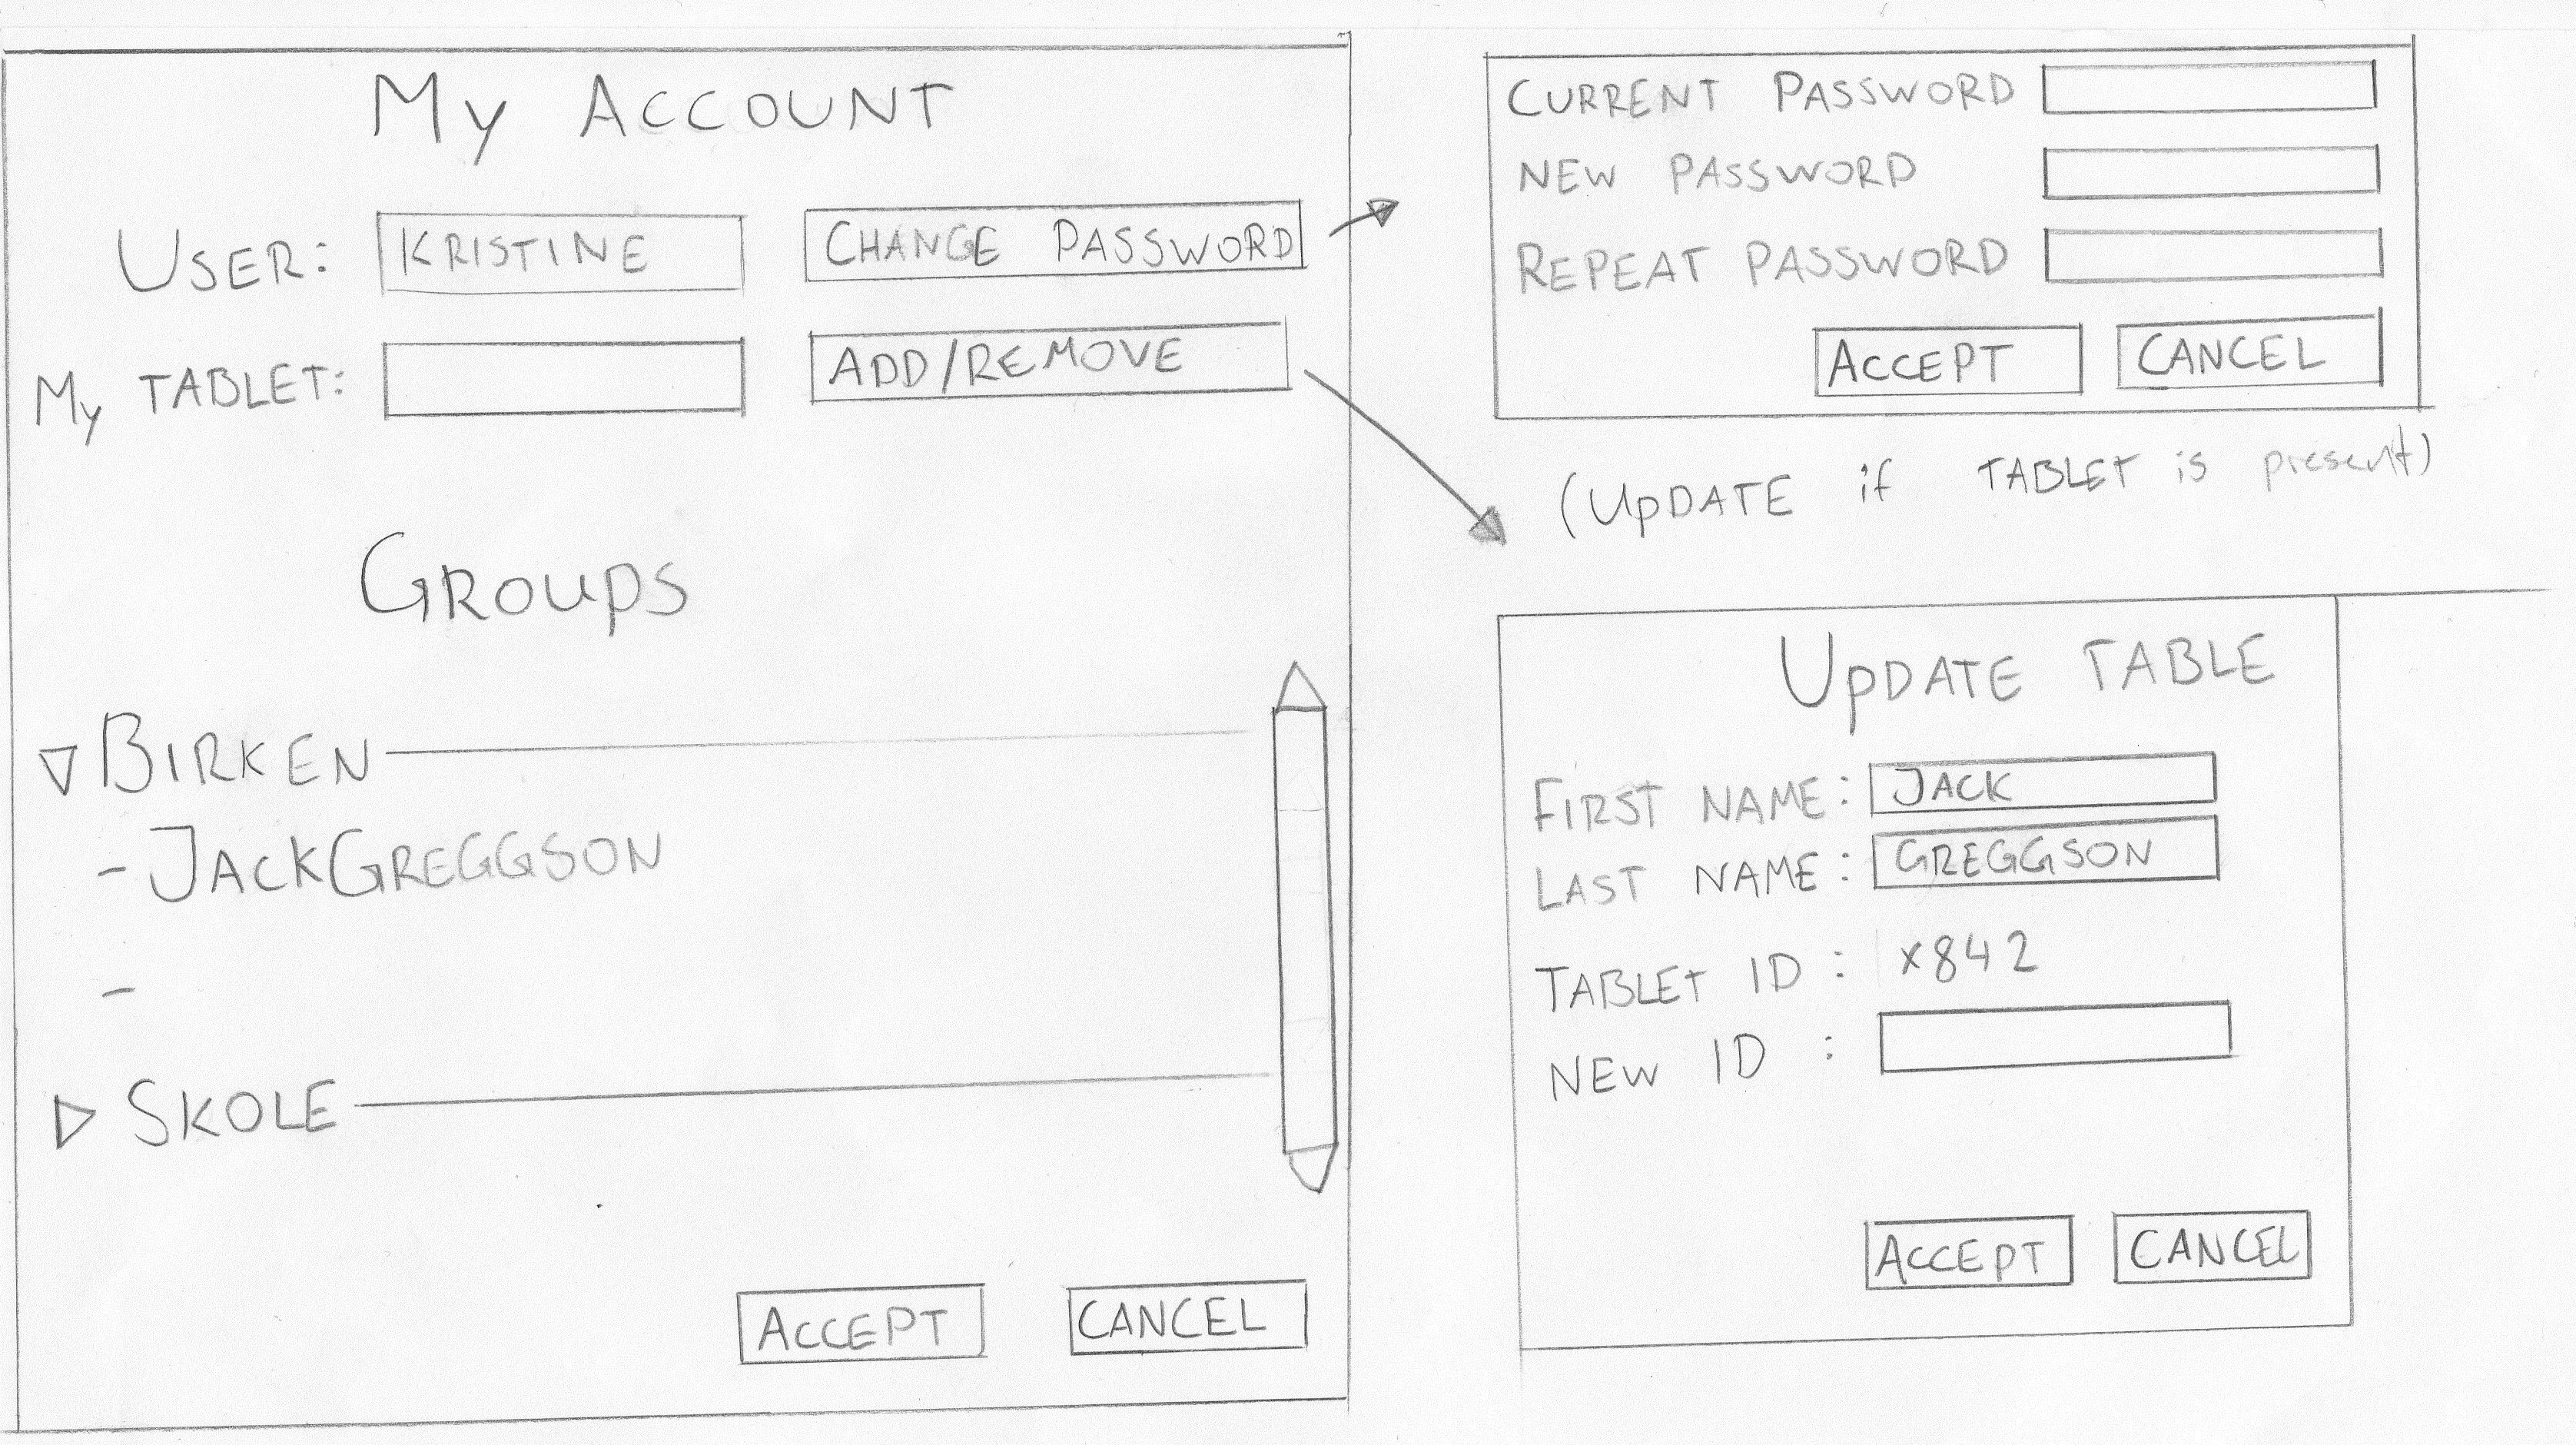
\includegraphics[width=1.00\textwidth]{img/myAccount.jpg}
	\caption{Design of My Account}
	\label{fig:myAccount}
\end{figure}


In this prototype design there is only one page and two pop up boxes, in the first the user can change his/hers password and in the other the user can add/update or delete a device. On the ``My Account'' page the user could also see or update devices in a group, creating confusion. This design was not thought through because the field ``My Tablet'' could be the user's own mobile device. In the beginning it was meant as his/hers child's mobile device and in both cases the user could have more than one mobile device, which should be registered, but is unavailable in this design. 

The group under ``My Account'' is needed because the user of this administration system could both have access to it privately and profecionally. For example the user coud be a parent to an autistic child and also a kindergarten teacher. This mean groups would be necessary when the user wants to change something on all but his/hers child's device without repeating the same process for each device in the kindergarten. The design is missing something that indicates how the user can add a device to a group. In the evaluation of this prototype it was also decided that ``My Account'' also should contain both the child's personal information and device settings. In the implementation it was decided that user information, group, child and child's device should be under different tabs.   
 
\section{The final design}
In the Figure \vref{fig:finalDesign} is the implemented design. It is very similar to the last paper prototype and the HTML prototype. The green menu will contain buttons with pictures and names of the children with connected devices. The pink menu will contain a list of the applications installed on the corresponding child's device. The contact book's design has been altered slightly, this alteration can be seen when the user creates a new message, where instead of opening in a light box window it unfolds when pressing the ``Nyt Indl�g'' label.  

\begin{figure}[!ht]
	\centering
		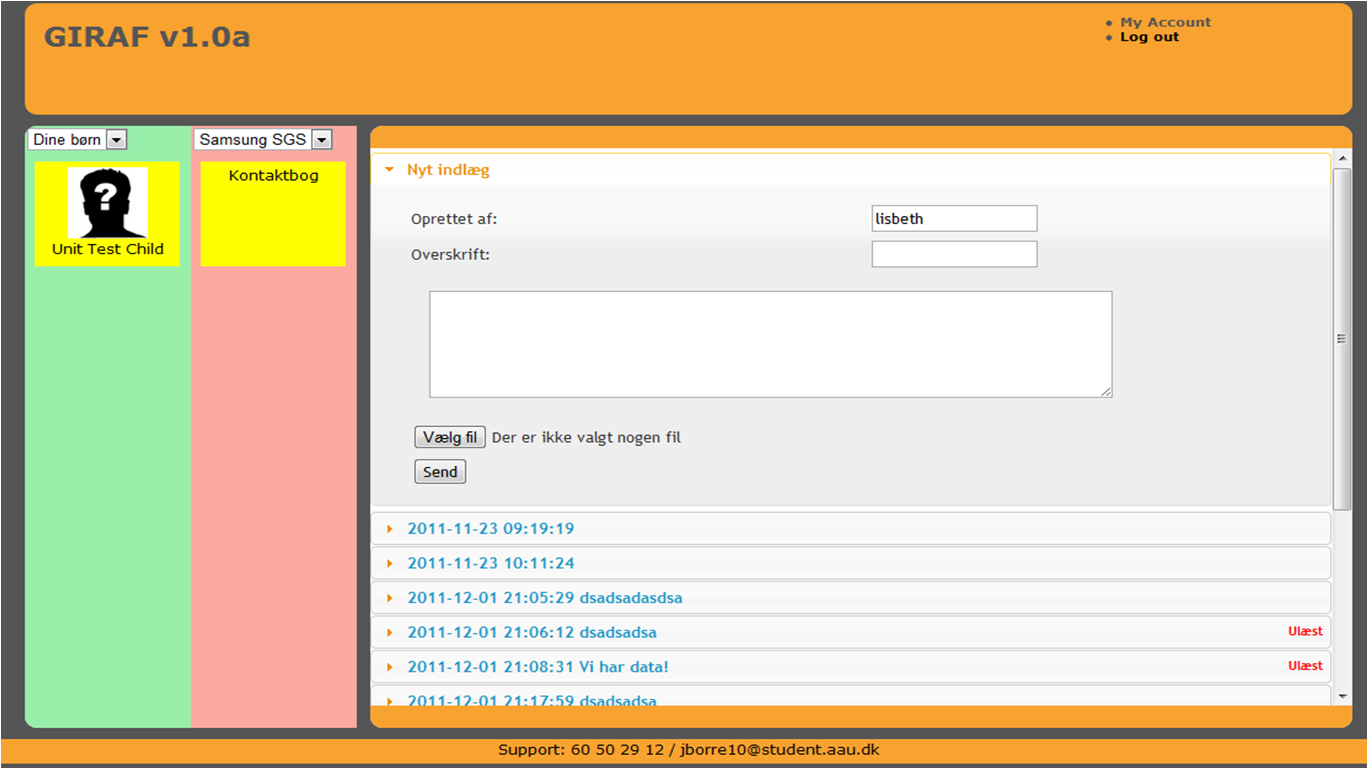
\includegraphics[width=1.00\textwidth]{img/finalDesign.png}
	\caption{Screenshort of the implemented design}
	\label{fig:finalDesign}
\end{figure}
